% This file should be replaced with your file with an thesis content.
%=========================================================================
% Authors: Michal Bidlo, Bohuslav Křena, Jaroslav Dytrych, Petr Veigend and Adam Herout 2019

\chapter{Introduction}
importance of GUI testing, goals, regressions, errors 

The goal of this work is to design and implement a tool for generating tests for GNOME desktop applications using AT-SPI metadata created as a by-product of an architecture supporting assistive technologies.

The architecture expose application as a tree of accessibility objects with their current state. Every object is defined by several properties and set of actions that can be invoked to change the current state. Since accessibility support has been implemented to very fundamental layers of GTK/GNOME framework (widget level), it provides a suitable way for development of automated test suites.\cite{pyatspi2} 

Modern GUI applications are being developed more rapidly with lack of proper regression testing. 

manual testing vs automation clanok


Additionally this effort should also help to reveal defects and missing parts in accessibility itself and improve the experience for users with disabilities.

\chapter{Accessibility}
Accessibility in general is a technology that helps people with disabilities to participate in essential life activities. Considering the accessibility as a part of GNOME desktop, it includes libraries and development tools allowing users with disabilities to use other options of interaction with GNOME desktop environment. Those options includes voice interfaces, screen readers and other alternative input devices.\cite{gnomeADG}
\section{The Accessibility Toolkit (ATK)}
Assistive technologies are receiving information from the Accessibility toolkit (ATK) which provides API built in to all GNOME widgets. Therefore, assistive technologies are able to automatically read most of the labels on screen without any extra efforts made by developers which is achieved by ATK, as it provides set of interfaces which are required to be implemented by GUI components. The interfaces are toolkit-independent, meaning that their implementation could be written for many widgets, including widgets from frameworks such as GTK\footnote{https://www.gtk.org/} and Qt\footnote{https://www.qt.io/}.
\section{GNOME Accessibility Implementation Library (GAIL)}
Majority of GNOME applications are written in GTK framework. The framework provides dynamically loadable module named GAIL with implementation of ATK interfaces for all GTK widgets. Once the module is loaded at runtime, the application is fully capable to cooperate with ATK without any further modifications.
GNOME desktop does not load accessibility support libraries by default, it has to be enabled by setting a special gsettings key which can be achieved either by dconf\footnote{https://wiki.gnome.org/Projects/dconf} editor or by execution of the gsetting command in terminal:
\begin{verbatim}
    gsettings get org.gnome.desktop.interface toolkit-accessibility true
\end{verbatim}
Additional configuration may be required for applications written in other frameworks such as QT or Java. Furthermore, implementations of other assitive technologies might be too application specific or use various techniques like OS event snooping etc. Compared to GNOME Desktop, all information required by assistive technologies (AT) are passed from GNOME Accessibility Framework to a toolkit-independent Service Provider Interface (SPI). The SPI is a key component providing stable and consistent2 API for screen readers, magnifiers, etc. Accessibility support is relying on per-toolkit implementation (GTK, QT, Java) and its APIs exported through relevant bridges to unified AT-SPI interface, as described on Diagram \ref{ATSPI_architecture}.

\begin{figure}[hbt]
	\centering
	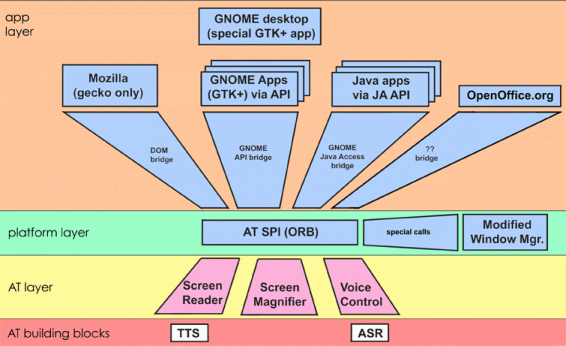
\includegraphics[width=1\textwidth]{obrazky-figures/GNOME_desktop_Accessibility.png}
	\caption{GNOME Accessibility Architecture overview}
	\label{ATSPI_architecture}
\end{figure}

The widget is accessible, if a developer use any GTK/GNOME widget and follows the general accessibility guidelines\footnote{https://developer.gnome.org/accessibility-devel-guide/stable/gad-coding-guidelines.html.en} with properly implemented ATK interfaces. Considering that the stock GTK/GNOME toolkit widgets have implementations of these interfaces provided, new widgets will inherit the functionality and gain suitable accessibility support as well. There is no need to make specific code changes to provide accessibility support altought application might alter some default descriptions and improve the user experience by describing them better, especially if widget is used for some specific purpose. The ATK provides set of functions to achieve this along with the ability to make any custom component accessible\footnote{https://developer.gnome.org/accessibility-devel-guide/stable/gad-custom.html.en}.\cite{accessibleWidgets}

\newpage
\section{pyatspi}
Package pytaspi is a Python wrapper around AT-SPI C implementation which loads the Accessibility typelib and imports the classes implementing AT-SPI interfaces.\cite{pyatspi}

The mode of application provided by AT-SPI can be described as a tree of widgets starting with a root element where every sub-element represent one running application on the GNOME desktop. Each application has zero or more children, each child is distinguishable by its position in the tree and several properties including:
\begin{itemize}
    \item name - for most widgets contains text identical with a text label visible on widget
    \item roleName - specifies the widget type
    \item childCount - number of sub-elements 
    \item actions - list of available action which can be performed by accessibility
    \item visible - boolean value, indicated that object is visible to the user
    \item showing - boolean value, object is rendered
    \item text -
    \item description - contains element description for users
    \item position - x, y coordinated on the screen (might be related to other component)
\end{itemize}

Additionally, elements can be linked together in other useful ways (except parent-child relationship) where labels are linked with widgets like text fields, check boxes, combo boxes etc. These labels are making widgets easier to find or interact with. Other advantageous properties like showing or visible can be used to decide whether elements are hidden from the active screen area, thus they are not available for interaction. Role names of elements are also important as some elements are offering some widgets specific methods like selecting values for radio buttons, selecting options in combo boxes or simple click method on buttons. Access to this functionality is focused in a singleton object named registry that provides services for subscribing to specific events and as mentioned before, generating mouse and keyboard events on demand.

pyatspi is an open source project available for most of Linux distributions via distro specific packaging services (package named python3-atspi) or can be built from its sources\footnote{https://gitlab.gnome.org/GNOME/pyatspi2}.

\section{Accerciser}
GUI tool for exploration of accessibility


\chapter{behave}
\chapter{GUI TESTING}
https://ldtp.freedesktop.org/wiki/
https://en.wikipedia.org/wiki/Linux_Desktop_Testing_Project
https://wiki.ubuntu.com/Xpresser/
AppStream data
\chapter{python}
\chapter{behave}
\chapter{verification}
\section{ATSPI}
\section{text recognition pytesseract}
\section{opencv2 - image comparison}